\section{\name's Architecture}
\label{sec:arch}

% {\color{blue} Points to cover:

% \begin{itemize}
%     \item The goal: decode weak transmission by collating information from multiple base-stations
%     \item Flow diagram (picture with cloudy and edgy stuff)
%     \item The strawman comparison: stream everything
%     \item Strawman limitations
%         \begin{itemize}
%             \item Weak signals and limited bandwidth (problems at gateways (could use joint decoding of preambles but cant afford to stream everything))
%             \item Scaling issues (problems at the cloud)
%         \end{itemize}
% \end{itemize}
% }

The goal of \name\ is to decode weak transmissions, which could not be
decoded by any individual gateway, by collating receptions from multiple
gateways at the cloud. At one level, this  enables us to expand network coverage area reaching clients deep inside buildings, underground or in outer reaches of the city. More fundamentally, it saves energy on the vast majority of client devices, even if they are within range of some gateways, by allowing them to increase their data rate without experiencing any loss in performance. Our results in Sec.~\ref{sec:energy-savings} demonstrate that lowering transmit time results in a direct and significant impact on battery life. 

Fig.~\ref{fig:architecture} depicts \name's architecture where we assume the gateways can be user-deployed  both indoors and outdoors, and cost a few hundred dollars. These base stations have an Ethernet backhaul to the cloud that accommodate a maximum uplink bandwidth of a few megabits per seconds. Much like the standard LoRaWAN architecture, MAC-layer scheduling is performed at the cloud with gateways relaying their received data to the cloud. However, to accommodate decoding weak received signals, we also allow gateways to ship raw received I/Q signals from feeble low-power clients to the cloud. The cloud aggregates such weak signals and coherently combines them to decode the underlying data bits from feeble receptions across multiple gateways. In other words, \name\ performs a joint optimization of the  PHY-layer at the cloud, simultaneously improving battery life and range of low-power clients at the expense of increased computation at the cloud. 

Yet, realizing a scalable and real-time system based on the above architecture is challenging both at the gateways and the cloud: 
\begin{itemize}
\item {\bf At the Gateway: } Firstly, given that signals from weak LP-WAN clients are often well below the noise floor, gateways are unaware of these packets in the received signal. This means that base stations must effectively send all their received raw signal data to the cloud to detect and decode weak signals, stressing their limited uplink bandwidth. 
\item {\bf At the Cloud: } Second, the cloud must identify signals from which gateways need to be combined to recover transmitted data from multiple clients. At city-scale, it is  conceivable that overlapping weak transmissions from different clients are received at the same time by gateways, making data recovery challenging at the cloud.
\end{itemize}


\begin{figure}[!htb]
    \centering
    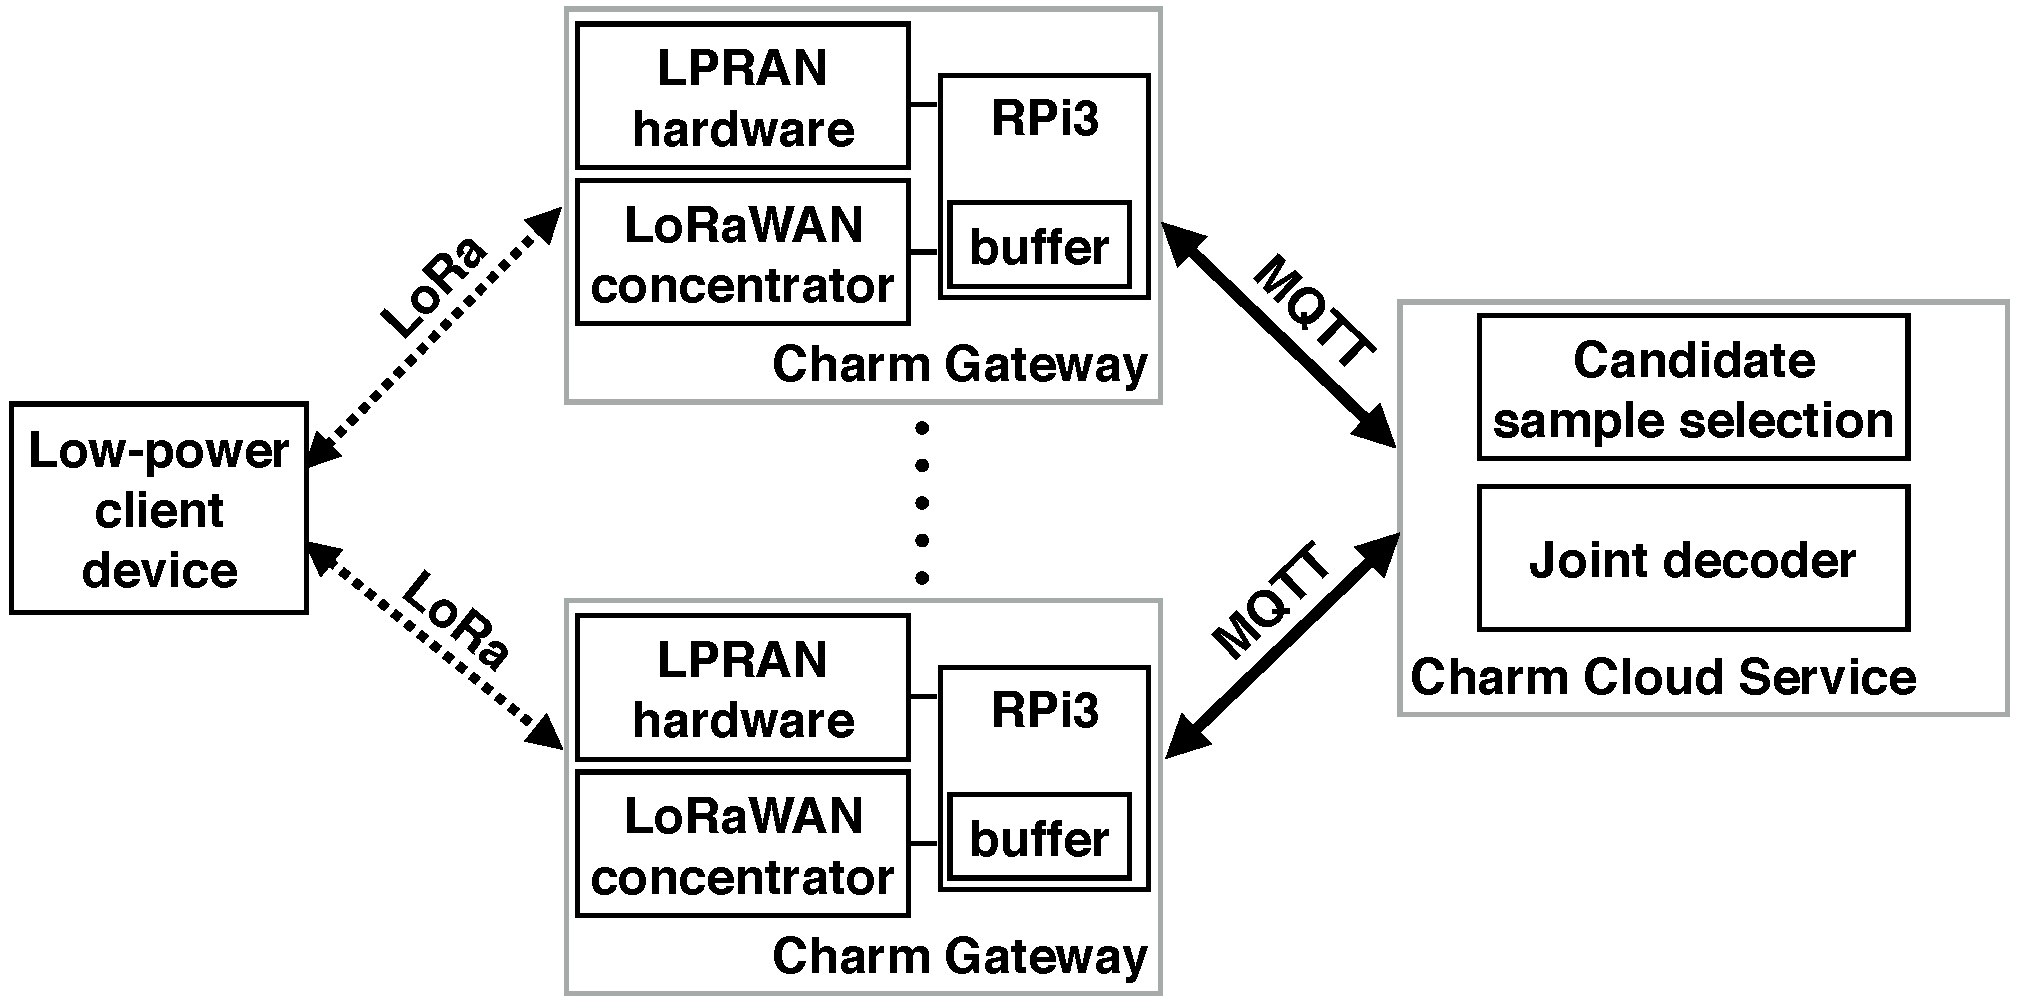
\includegraphics[width=0.45\textwidth]{figures/charm-architecture_cropped.pdf}
    \caption{Architecture of \name}
    \label{fig:architecture}
    \compactimg
\end{figure}


 The rest of this paper describes \name's solutions to each of these challenges. Specifically, \name\ makes two key contributions: (1) A software interface at the gateway to identify weak transmissions to ship to the cloud, and a hardware design that facilitates these decisions in real-time; (2) A scalable cloud based PHY-layer processing system at the cloud that operates at city-scale. Next we elaborate on each of these components. 




% Some of the transmission our system aims to decode, have signal power as low
% as -30 dBm below the noise floor. Such transmission are not only impossible to
% decode for an individual gateway, but they are also difficult to detect .
% Since transmitted signals would combine coherently, contrasted to random noise
% that combines non-coherently, an appropriate combination of radio streams
% from different gateways might be able to decode such a message.

% \subsection{Continuous streaming}
% \label{sec:continuus-streaming}

% A solution, similar to Cloud-RAN \cite{chen2011c}, is to continuously
% stream all radio data to a cloud-based joint decoder. The gateways then act as
% simple forwarders while all decisions and processing is done by a capable and
% scaleable cloud server. This architecture is similar to LoRaWAN, but for the
% physical layer. Additionally, joint detection of packets might detect even
% weaker packets that what is detectable by a single receiver.

% However, streaming raw radio I/Q data streams to the cloud at each base
% station suffers from two major issues: (1) They require high bandwidth
% connectivity between gateways and the cloud decoder -- typically a fiber-optic
% backhaul. Indeed, streaming LoRaWAN raw signal data at its lowest bandwidth
% to the cloud would incur 18 Mbps of uplink bandwidth. This is far too
% expensive and wasteful, given the limited uplink bandwidth at
% consumer-deployed LoRaWAN gateways which are often just home set-top boxes.
% (2) Processing large amounts of data at the cloud poses a scalability
% challenge with an increasing number of gateways.

% %2.250 MBps

% % Swarun



% % {\color{blue} Describe the entire story in this section}

% Note: continuous streaming data rate 2.250 MBps for 8 channel gateways

% \subsection{Selective aggregation}
% \label{sec:selective-aggregation}

% A: LoRa packets have this nice characteristic of having a very long header. We could detect packets locally and only stream detected chunks to the cloud

% Q: Our network is very vast and performance degrades near the boundaries, which also cover the most area. At any point of time there will always be many struggling transmitters.
